% 2nd - Preprocessing
%% Includes: representation, neighbourhood, viewpoint transformations, noise filtering, segmentation, keypoint detection
\chapter{Pre-processing}
\label{cha:preproc}

This chapter describes basic RGB-D image processing tool set, that prepares an input image for extracting relevant information during object recognition.

%---------------------------------------------------------------------------

\section{Representation}
\label{sec:representation}


%rgb-d, point clouds, tsdf
%algos for conversion, timing

Depth and colour information of the environment can be represented in computer memory by the means of various data structures, which differ in their complexity and applicability. In case of typical, low-cost RGB-D cameras, the raw data that is retrieved from the device firmware and operating system drivers come in a form of two images, one from a conventional colour camera and the other from the depth sensor, as depicted on Figure x.

Figure XXX - drawing of camera with 2 raycasts, 2 images

Data retrieved from a depth sensor have a form of one channel, two dimensional image. Each pixel contains measurement of the distance between depth camera reference frame origin and a corresponding point on the reflected surface. In case of Asus Xtion sensor, this data is stored as 32 bit floating point values. It is important to note, that depending on the acquisition method, not all of the surface point distances are measured. For example, if the surface is translucent, most sensors will fail to retrieve proper distance. Such situation is reflected in data by the use of \textit{Not a Number (NaN)} pixel values.

Due to the displacement between color and depth sensor [reference], RGB-D cameras require a calibration step to align the measurements. For this purpose, open source packages such as [XXX] can be used. Finally, successful RGB-D data alignment yields a four channel digital image, which can be defined more formally as:
\begin{equation}
\label{eq:rgbdimage}
I: \{1,\dots,M\} \times \{1,\dots,N\} \rightarrow [0,1]^4,\qquad I(u,v) =  \begin{bmatrix} I_R(u,v) \\ I_G(u,v) \\ I_B(u,v) \\ I_D(u,v) \end{bmatrix},
\end{equation}
where:
\begin{itemize}
\item $M \in \mathbb{N}$, $N \in \mathbb{N}$ - row and column image size,
\item $I_R(u,v), I_G(u,v), I_B(u,v)$ - red, green and blue colour channel intensities,
\item $I_D(u,v)$ - depth channel intensity
\end{itemize}

RGB-D image formulation \ref{eq:rgbdimage} is mostly suitable for per channel, classic two-dimensional image processing, such as applying morphological operators or linear filters [XXXImProc]. It does, however, limit the three dimensional surface information to a single viewpoint, which is undesirable for some applications in robotics, especially for object modelling and environment mapping. A generalized data representation that overcomes this limitation is called a \textit{point cloud}. It can be defined as a point set $C \subset \mathbb{R}^N$ of $N$-dimensional vectors. Depending on the usage, the points can represent different image modalities and features, such as point location in some reference frame, colour, surface normal vector or more advanced descriptors (see chap. \ref{cha:feature}). Direct conversion from a depth map to point cloud, requires projective transformation [XXX] of the depth channel to render Cartesian $x,y,z$ point coordinates in camera reference frame. In this manner, multiple RGB-D image frames, taken from different viewpoints can be stored within a single point cloud, by registering their points to a common coordinate system.

There are other possible representations of depth data. In contrast to point clouds, \textit{Patch volumes} [XX] and \textit{Signed distance functions} are dense representations of the three-dimensional environment, where each point represents distance to the nearest surface. Patch volumes use BLABLABLA. OctoMaps use BLABLABLA. Those representations, however, are mainly used for environment mapping and SLAM applications. This work will further focus on point clouds, as they are the most covered representation for object recognition. ??

%TODO: model format

%---------------------------------------------------------------------------

\section{Neighbourhood}
\label{sec:neighbourhood}

Similarly to classical image processing, a wide range of point cloud processing algorithms rely on the notion of point neighbourhood. Given a metric function $d$ and a query point $p_q$ in the point cloud $P$, two commonly used types of neighbourhoods can be defined. A \textit{r-neighbourhood} is a set composed of all the points $p_i \in P$ that lie within a sphere of a radius $r$ and a center in $p_q$, thus satisfying the condition
\begin{equation}
d(p_	q, p_i) \leq r.
\end{equation}
The other type is \textit{k-neighbourhood}, a set of $k$ nearest points in the sense of given metric. Proper determination of neighbourhood size parameters, either $r$ or $k$ correspondingly, is crucial in further analysis. Too small values do not provide enough information about the surface. Too large, on the other hand, will average the surface and skip small details. Complexity and efficiency of neighbourhood search depends on different internal data representation in a point cloud.

From computational point of view, a point cloud that is directly converted from RGB-D image can be internally stored in a two dimensional array of points, with elements corresponding to image pixels. Point clouds with such data arrangement are commonly referred to as \textit{organized}. Image-like ordering is beneficial, because it reflects the spatial distribution of points directly into memory.


Also known as support.
Organized neighbourhoods.
KD-tree.
Flann.
\textit{“scale” corresponds to the “support radius” (TombariA et al, 2013)}
%---------------------------------------------------------------------------

\section{Surface normals}
\label{sec:normals}

Many of the algorithms used further during the analysis of a point cloud base on the notion of a surface normal, known from the 3D geometry. These vectors are also widely used for shading in 3D computer graphics and a variety of methods have already been developed to solve the surface normal estimation problem. One of the simplest uses the least-squares plane fitting to estimate the normal to a plane tangent to the surface, which approximates the desired vector \cite{rusuthesis}. More specifically, for a given point on the surface, it's $k$-neighbourhood centroid $\bar{p}$ is calculated as:
\begin{equation} 
\bar{p} = \frac{1}{k} \cdot \sum\limits_{i=1}^{k} p_i 
\end{equation}
The tangent plane is thereafter defined by the centroid $\bar{p}$ and the sought normal vector $\vec{n}$. The latter is computed by minimizing the total distance from every k-neighbour $p_i$ to the tangent plane, given by $\sum\limits_{i=1}^{k} (p_i - \bar{p})\cdot \vec{n}$. The minimization problem can be solved by utilizing the covariance matrix $C \in \mathbb{R}^{3x3}$, given by:
\begin{equation}
C = \frac{1}{k-1}\sum\limits_{i=1}^{k}(p_i - \bar{p})\cdot (p_i - \bar{p})^\intercal
\end{equation}
The covariance matrix $C$ is symmetric, positive semi-definite and possess three real eigenvalues $\lambda_j \geq 0, i = 1,2,3$. The eigenvector corresponding to the smallest eigenvalue is an approximation of the desired normal vector $\vec{n}$, disregarding the sign. Furthermore, if the viewpoint $v_p$ is known, the normal $\vec{n}$ has to be oriented towards  $v_p$, which means that it has to satisfy the condition:
\begin{equation}
\vec{n}\cdot(v_p-p_i) > 0
\end{equation}


Processing time. Cuda implementation. Complete solution used \cite{eigenvalues3x3}.

Example PCD with normals:
\begin{figure}[h]
\centering
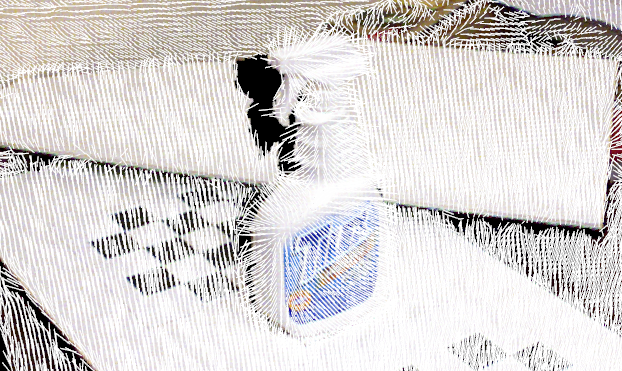
\includegraphics[width=0.8\textwidth]{fig/Normal}
\caption{ Normals }
\label{fig:normals}
\end{figure}

\section{Noise filtering}
\label{sec:noise}

%TODO: types of noise
Types of noise, frequency response, low pass filtering, nonlinear filtering

%TODO: boundary
Boundary estimation

%TODO: clutter
Occlusion and clutter from Guo

One of the most important stages of data preprocessing is the filtration. Probably the most basic point cloud filter is the pass-through filter, which reject all points outside a given range along a specified dimension. This procedure allows to focus the analysis process on the region of interest, i.e. the reachable workspace of a manipulator. Apart from limiting the cloud dimensions, the number of data points can be also reduced by downsampling. The voxel grid filter is typically used for this purpose. This filter creates a three dimensional regular grid over the input point cloud data and then, in each voxel, approximates all the present data points with their centroid. Such reduction is particularly useful when large point cloud datasets have to be processed online with limited computing resources. Finally, the filtration process has to cope with numerous measurement errors present in the raw data acquired from the 3D camera. Such measurement noise 
manifests itself in the form of sparse outliers, which corrupt the results of further processing, i.e. the surface normals estimation. The impact of those irregularities can by reduced by applying an outlier removal filter. The simplest form of such filter rejects all the data points which does not have enough neighbours within a specified radius. A more refined version is based on the neighbouring points distance distribution. Firstly, the mean distance from each point to all its neighbours is calculated. Next, based on the assumption that the resulting distribution is Gaussian, all the points whose mean distances lay outside of an interval defined by the global distances mean and their standard deviation are rejected from the dataset. The effects of statistical outlier removal are presented in the Figure \ref{fig:outlierremoval}.

%---------------------------------------------------------------------------
